\documentclass[a4paper, 12pt]{article}
% math symbols
\usepackage{amssymb}
\usepackage{amsmath}
\usepackage{mathrsfs}
\usepackage{physsummer}


\usepackage{enumitem}
\usepackage[margin = 2cm]{geometry}

\tolerance = 1000
\emergencystretch = 0.74cm



\pagestyle{empty}
\parindent = 0mm

\begin{document}

\setphysstyle{ГЦФО 8}{Серия Ш-05}{12.10.2016}

\Large
\setcounter{notask}{15}

\taskpic{ Тонкостенный сосуд массы $m$, расположенный вертикально вниз
  дном, плавает на границе раздела двух жидкостей с плотностями
  $\rho_1$ и $\rho_2$. Найти глубину погружения стакана в нижнюю
  жидкость, если дно стакана имеет толщину $h$ и площадь $S$. Массой
  стенок стакана пренебречь. }
{
  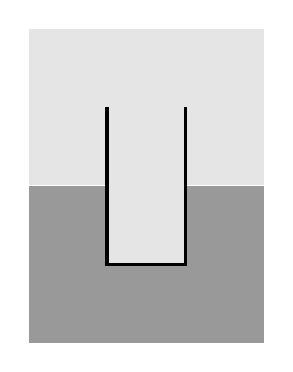
\begin{tikzpicture}
    \draw[draw=white, fill=gray!20] (0,3) rectangle ++(3,-2);
    \draw[draw=white, fill=gray!80] (0,1) rectangle ++(3,-2); 
    \draw[draw=gray!20, fill=gray!20] (1,2) rectangle ++(1,-2);
    \draw[very thick] (1,2) -- ++(0,-2) -- ++(1,0) -- ++(0,2);    
  \end{tikzpicture}
}
% НГУ-1, 1.146

\task{ Цилиндрический сосуд заполнен двумя неперемешивающимися
  жидкостями с плотностями $\rho_1$ и $\rho_2$. В жидкость погружается
  куб с ребром $l$. Найти глубину погружения куба в жидкость с
  плотностью $\rho_2$, если плотность вещества куба равна $\rho$
  ($\rho_2 > \rho > \rho_1$). }
% НГУ-1, 1.147

\task{ На дне сосуда на одной из своих боковых граней лежит
  треугольная призма. В сосуд налили жидкость плотности $\rho_0$,
  причём её уровень сравнялся с верхним ребром призмы. Какова
  плотность материала призмы, если сила давления призмы на дно сосуда
  увеличилась в три раза? Жидкость под призму не подтекает. }
% НГУ-1, 1.152

\end{document}


%%% Local Variables: 
%%% mode: latex
%%% TeX-engine:xetex
%%% TeX-PDF-mode: t
%%% End:
